%% NUMERICAL TESTING OF THE CRITERIA
%%

\subsection{Overview}

Starting from three physically imposed conditions for the intensity profile of a
limb darkened star, we have derived seven criteria which bound the three LDCs
parameterizing the \citet{sing:2009} limb darkening law. In this section, we
test the validity of these criteria in terms of i) completeness and ii) 
validity. We define these terms as follows:

\begin{itemize}
\item[{\tiny$\blacksquare$}] \textbf{Completeness:} A fully complete set of 
criteria require that the loci of points for which the physical conditions are
met also satisfy our seven criteria.
\item[{\tiny$\blacksquare$}] \textbf{Validity:} A fully valid set of criteria 
requires that that the loci of points which meet our seven criteria 
never break the two physical conditions.
\end{itemize}

These two tests can be thought of in the following way. Incomplete cases imply 
that our criteria are overly-conservative, cropping some parts of physically 
plausible parameter space. Invalid cases imply that our criteria are
overly-optimistic, erroneously predicting that some parts of parameter space are
physically plausible.

\subsection{Completeness Tests}

We perform our tests via numerical Monte Carlo simulation. We begin by
drawing a uniform random point in the parameter space $\{c_2,c_3,c_4\}$. The 
expected upper and lower bounds on these terms were calculated earlier in 
\S\ref{sub:c4c2plane}. We begin by using these bounds except that we use the 
original $c_4>-1$ constraint rather than the modified criterion F. We then
take this cuboid and double the lengths of each side such that we consider
the ranges: $-9/2<c_2<27/2$, $-3(4+3\sqrt{2})<c_3<(4+3\sqrt{2})$ and
$-6<c_4<14$. These adjustments are made to ensure that we explore the full
range of physically allowed LDCs during this test.

A sample point is drawn from this cuboid and then tested as to whether the 
physical conditions \I, \II\ and \III\ are met. In practice, we accomplish this 
by computing $10^3$ points along the functions $I(\mu)$ and 
$\partial I(\mu)/\partial\mu$ varying $\mu$ from $0$ to $1$ in equal, linear 
steps. For \III\ we simply test if $c_3<0$, since this condition only applies
at the location $\mu\to0$. If the physical conditions are not met, then we 
generate a new trial point. If they are met, then we proceed to test if 
the analytic criteria A to G are satisfied for this accepted point.

In total, we repeat this process until $10^4$ accepted points are found, 
requiring $\sim10^7$ simulations in total. Although the number of simulations 
may appear modest, we note that at each realization we must numerically compute 
the functions $I(\mu)$ and $\partial I(\mu)/\partial\mu$ at $10^3$ locations, 
which takes substantial computational overhead ($\sim30$\,s per simulation).

We find that $95.3$\% of the accepted points also satisfy criteria A to G, or
a completeness of $>95$\%. This indicates that our seven criteria are slightly
overly-conservative, cropping $\sim5$\% of the physically permissible 
LDCs. If we use the unmodified versions of criteria F and G (see 
\S\ref{sub:criterionF} and \S\ref{sub:criterionG}) and repeat the exercise,
we find that $100$\% of the physically valid points satisfy the criteria.
However, as discussed in \S\ref{sec:transformations}, this now yields an
asymmetric loci of allowed LDCs, impeding efforts to find an efficient sampling
algorithm.

\subsection{Validity Tests}
\label{sub:validitytests}

In an analogous approach to the previous tests, we begin by drawing uniform 
random samples in $\{c_2,c_3,c_4\}$ as before, except that we know constrain the 
cuboid to the specific bounds derived in \S\ref{sub:c4c2plane} (including 
$c_4>0$). We then test whether the seven analytic criteria are satisfied or not 
and if so consider the point to be accepted. We continue until $10^6$ accepted 
points are found, which we found required $101,163,869$ trials. Since we used 
the tightest bounding cuboid possible here, this reveals that the most efficient
sampling possible without transforming the $\{c_2,c_3,c_4\}$ LDCs would be
just under 1\%. Whilst one could proceed in this way, applying an 
acceptance/rejection test at each realization, uniform sampling would reject
over 99\% of realizations, making such an approach highly inefficient.

We next test whether each of these accepted points satisfies the physical
conditions \I, \II\ and \III. As before, this is done by evaluating the 
functions $I(\mu)$ and $\partial I(\mu)/\partial\mu$ at $10^3$ evenly spaced 
locations.

From these tests, we find that 100\% of the $10^6$ accepted points satisfy the
physical criteria. Therefore, the seven criteria are fully valid and drawing
a point which satisfies them is guaranteed to always satisfy the physical 
conditions \I, \II\ and \III.

These tests therefore confirm that our criteria have a very high completeness
and perfect validity. We therefore proceed with confidence that
they provide a suitable set of constraints to evaluate the range of physically
plausible LDCs.

%%% 3D plot of the c-space
\begin{figure}
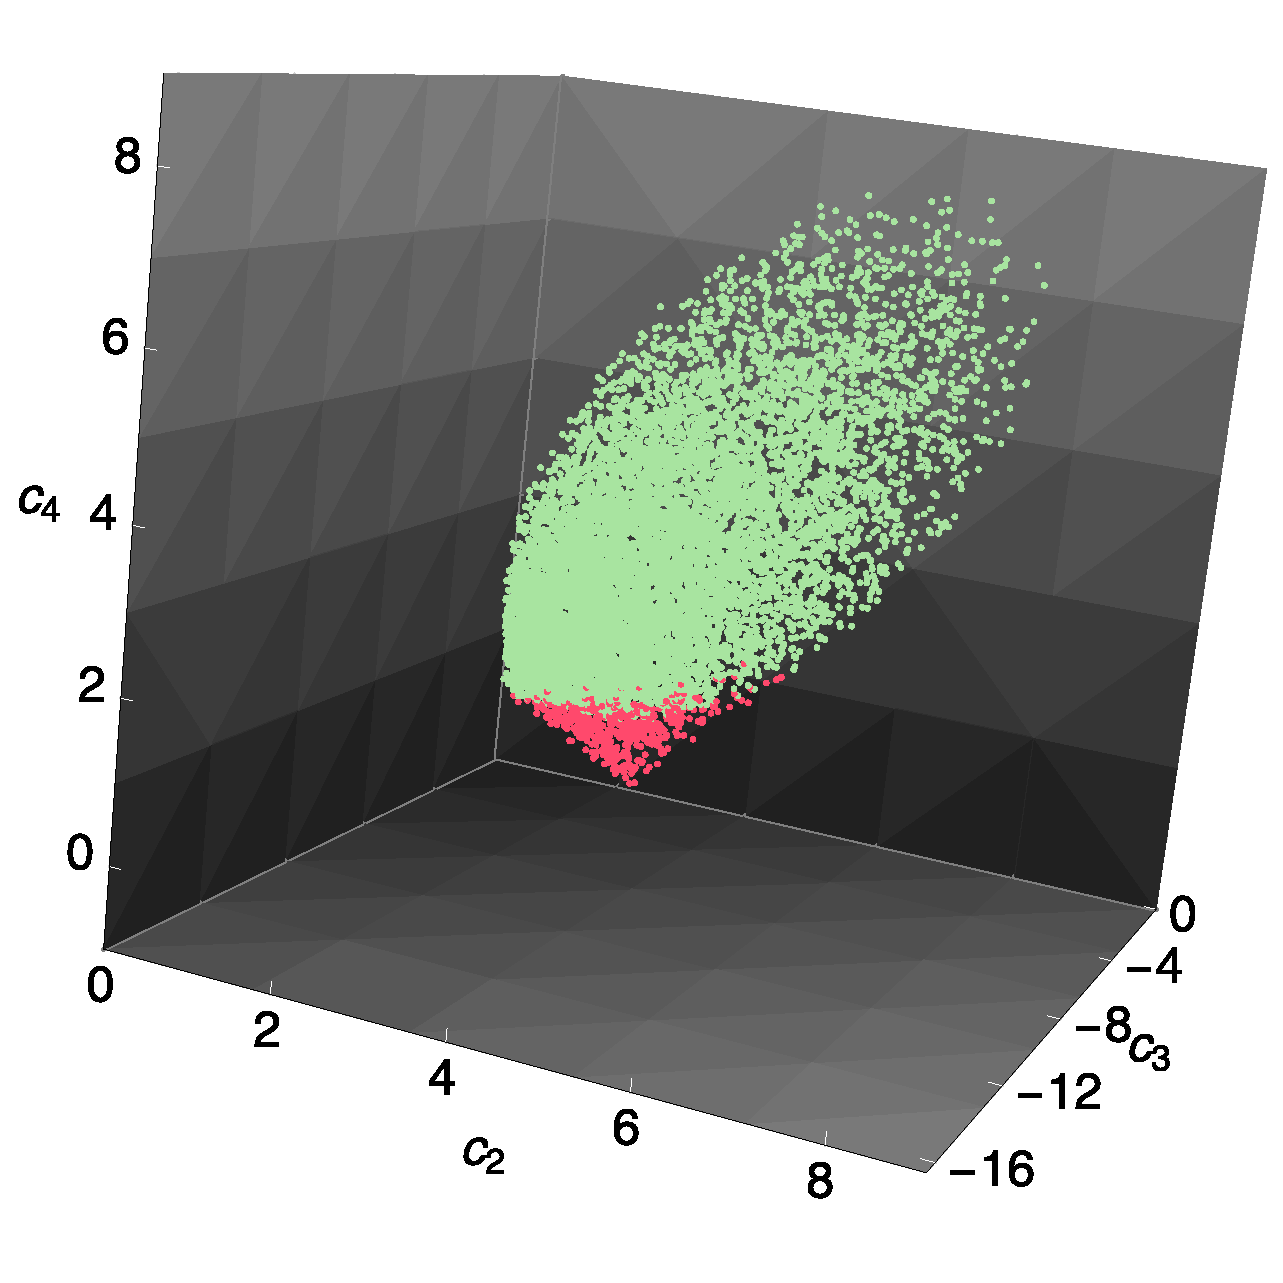
\includegraphics[width=\columnwidth]{c3Dplot.eps}
\caption{
3D plot of the allowed LDCs in the original parameter space: $\{c_2,c_3,c_4\}$. 
All of the plotted points satisfy the physical conditions \I, \II\ and \III,
as well as the unmodified criteria A-G. The green points also satisfy the 
modified criteria A-G (whereas the red do not), chosen to yield a more symmetric 
loci of points and comprising $>95$\% of the volume.
}
\label{fig:c3Dplot}
\end{figure}

